\section{BRST Quantization}

BRST quantization is a powerful algebraic method that allows one to systematically find the complete gauge-fixed action entering the path integral, thoroughly incorporating both the necessary ghost fields and the gauge-fixing terms. It is widely recognized by extending the key features observed in simpler examples, and it fundamentally utilizes the continuous BRST symmetry as a robust guiding principle. Eventually, this is a quantization method which is structurally similar to the Faddeev-Popov procedure, but mathematically more rigorous and generalized.

We illustrate the main, essential steps of the method using a non-Abelian Yang-Mills gauge theory as our primary example. The BRST quantization procedure strictly begins with the formal definition of the BRST symmetry. Starting directly from the original gauge-invariant lagrangian, one introduces anticommuting ghost fields physically associated with the original gauge symmetry. The essential, dynamical part of the BRST transformation rules is then determined by strictly imposing the algebraic requirement of nilpotency. Then, to properly implement gauge fixing, one adds an appropriate set of non-minimal auxiliary fields and constructs the complete gauge-fixed total lagrangian by selecting a suitable "gauge-fixing fermion". This elegant framework allows for a wide variety of gauge choices, proving its versatility. The key, indispensable ingredient throughout the entire procedure is the absolute nilpotency of the BRST symmetry operator.

Let us explicitly exemplify this within non-abelian gauge theories. One starts from the standard, classically gauge-invariant lagrangian
\begin{equation} \label{eq:45}
    \mathcal{L} = \frac{1}{2g^2}\text{tr}(F_{\mu\nu}F^{\mu\nu}) = \frac{2}{g^2}\text{tr}\left(\frac{1}{4}F_{\mu\nu}F^{\mu\nu}\right)
\end{equation}
for the Lie-algebra valued gauge field \(A_\mu(x) = -iA_\mu^a(x)T^a\). The classical infinitesimal gauge symmetry of the action is given by the local transformation
\begin{equation} \label{eq:46}
    \delta A_\mu(x) = D_\mu\alpha(x) \, .
\end{equation}

At this point, the BRST symmetry on \(A_\mu(x)\) is properly defined by introducing the ghost field \(c(x) = -ic^a(x)T^a\) and systematically replacing \(\alpha(x) \rightarrow \Lambda c(x)\) within the infinitesimal gauge transformation, where \(\Lambda\) represents the rigid, anticommuting Lie parameter defining the BRST symmetry\footnote{The covariant derivative of a field in the adjoint representation is \(D_\mu \alpha = \partial_\mu \alpha + [A_\mu, \alpha]\), and similarly \(D_\mu c = \partial_\mu c + [A_\mu, c]\). Additionally, the coupling constant is conventionally absorbed into \(A_\mu\) and \(c\).}. Evidently, the BRST symmetry operating on the gauge field is functionally equivalent to a pure gauge transformation.

The classical infinitesimal gauge transformation and its corresponding BRST transformation are given by:
\begin{equation} \label{eq:47}
    \delta A_\mu(x) = D_\mu \alpha(x) \quad \rightarrow \quad \delta_B A_\mu(x) = \Lambda D_\mu c(x)
\end{equation}

\begin{proof}
    The infinitesimal gauge transformation of the gauge field is defined as:
    \[
        \delta A_\mu(x) = D_\mu \alpha(x) = \partial_\mu \alpha(x) + [A_\mu(x), \alpha(x)]
    \]
    To construct the BRST symmetry, we replace the infinitesimal gauge parameter \(\alpha(x)\) with \(\Lambda c(x)\), where \(c(x)\) is the Grassmann-odd ghost field and \(\Lambda\) is a rigid (constant), anticommuting Lie parameter. Substituting this into the covariant derivative yields:
    \[
        \delta_B A_\mu(x) = D_\mu (\Lambda c(x)) = \partial_\mu (\Lambda c(x)) + [A_\mu(x), \Lambda c(x)]
    \]
    Since \(\Lambda\) is a global constant, it factors out of the partial derivative: \(\partial_\mu (\Lambda c) = \Lambda \partial_\mu c\). Furthermore, because \(\Lambda\) is a parameter that commutes with the Lie algebra generators \(T^a\) (acting only as a scalar coefficient in the color space), we can factor it out of the commutator as well: \([A_\mu, \Lambda c] = \Lambda [A_\mu, c]\). Therefore, we obtain:
    \[
        \delta_B A_\mu(x) = \Lambda \partial_\mu c(x) + \Lambda [A_\mu(x), c(x)] = \Lambda \big( \partial_\mu c(x) + [A_\mu(x), c(x)] \big) = \Lambda D_\mu c(x)
    \]
    which exactly reproduces the right-hand side of Eq. (\ref{eq:47}).
\end{proof}

Because it takes the form of a gauge transformation, the classical action is manifestly BRST invariant. Having introduced the dynamical ghost \(c\), we uniquely have to find its specific BRST variation, which is strictly obtained by requiring that the BRST transformation of the physical gauge field \(A_\mu\) be nilpotent.

The nilpotency of the BRST transformation on the gauge field uniquely determines the BRST transformation of the ghost field:
\begin{equation} \label{eq:48}
    [\delta_B(\Lambda_1), \delta_B(\Lambda_2)] A_\mu(x) = 0 \quad \rightarrow \quad \delta_B c(x) = -c(x)c(x)\Lambda
\end{equation}

\begin{proof}
    It is extremely useful to factor out the constant parameter \(\Lambda\) by introducing the Slavnov operator \(s\), such that \(\delta_B = \Lambda s\). Here, \(s\) is a Grassmann-odd (anticommuting) derivation, while \(\delta_B\) is a bosonic (commuting) operator.

    Let \(\delta_1 \equiv \delta_B(\Lambda_1)\) and \(\delta_2 \equiv \delta_B(\Lambda_2)\). Since \(\delta_1\) is bosonic, it obeys the standard Leibniz rule. Applying the commutator to \(A_\mu\), we find:
    \[
        \begin{aligned}
            \delta_1 (\delta_2 A_\mu) & = \delta_1 (\Lambda_2 s A_\mu) = \Lambda_2 \delta_1 (s A_\mu) \quad                                        &  & \text{(since \(\Lambda_2\) is constant)}            \\
                                      & = \Lambda_2 (\Lambda_1 s) (s A_\mu) = \Lambda_2 \Lambda_1 s^2 A_\mu = -\Lambda_1 \Lambda_2 s^2 A_\mu \quad &  & \text{(since \(\Lambda_1, \Lambda_2\) anticommute)}
        \end{aligned}
    \]
    By swapping the indices, \(\delta_2 \delta_1 A_\mu = \Lambda_1 \Lambda_2 s^2 A_\mu\). Thus, the commutator is:
    \[
        [\delta_1, \delta_2] A_\mu = \delta_1 \delta_2 A_\mu - \delta_2 \delta_1 A_\mu = -2 \Lambda_1 \Lambda_2 s^2 A_\mu
    \]
    Requiring \([\delta_1, \delta_2] A_\mu = 0\) is therefore strictly equivalent to requiring the nilpotency of the Slavnov operator: \(s^2 A_\mu = 0\).

    Now, let us compute \(s^2 A_\mu\) explicitly. We know that \(s A_\mu = D_\mu c = \partial_\mu c + [A_\mu, c]\). Applying \(s\) again, and remembering that \(s\) acts as an odd derivation (meaning \(s(AB) = (sA)B + (-1)^{|A|}A(sB)\)), we get:
    \[
        \begin{aligned}
            s^2 A_\mu & = s(D_\mu c) = s \big( \partial_\mu c + A_\mu c - c A_\mu \big)       \\
                      & = \partial_\mu(sc) + (s A_\mu)c + A_\mu (sc) - (sc)A_\mu - c(s A_\mu)
        \end{aligned}
    \]
    Notice that the terms involving \(sA_\mu\) form an anticommutator, while the terms involving \(sc\) form a commutator:
    \[
        \begin{aligned}
            s^2 A_\mu & = \partial_\mu(sc) + [A_\mu, sc] + (s A_\mu)c + c(s A_\mu) \\
                      & = D_\mu(sc) + \{s A_\mu, c\} = D_\mu(sc) + \{D_\mu c, c\}
        \end{aligned}
    \]
    Let us explicitly expand the anticommutator \(\{D_\mu c, c\} = (D_\mu c)c + c(D_\mu c)\):
    \[
        \begin{aligned}
            (D_\mu c)c & = (\partial_\mu c + A_\mu c - c A_\mu)c = (\partial_\mu c)c + A_\mu c^2 - c A_\mu c \\
            c(D_\mu c) & = c(\partial_\mu c + A_\mu c - c A_\mu) = c(\partial_\mu c) + c A_\mu c - c^2 A_\mu
        \end{aligned}
    \]
    Summing these two expressions, the \(c A_\mu c\) terms cancel out perfectly:
    \[
        \{D_\mu c, c\} = (\partial_\mu c)c + c(\partial_\mu c) + A_\mu c^2 - c^2 A_\mu = \partial_\mu(c^2) + [A_\mu, c^2] = D_\mu(c^2)
    \]
    Substituting this back into our expression for \(s^2 A_\mu\), we find:
    \[
        s^2 A_\mu = D_\mu(sc) + D_\mu(c^2) = D_\mu(sc + c^2)
    \]
    For the BRST transformation to be nilpotent (\(s^2 A_\mu = 0\)) for any arbitrary gauge field configuration, the argument of the covariant derivative must vanish identically:
    \[
        sc + c^2 = 0 \quad \implies \quad sc = -c^2
    \]
    Finally, translating this back to the BRST variation \(\delta_B = \Lambda s\), we obtain:
    \[
        \delta_B c(x) = \Lambda s c(x) = \Lambda (-c(x)c(x)) = -c(x)c(x)\Lambda
    \]
    which perfectly reproduces the right-hand side of Eq. (\ref{eq:48}).
\end{proof}

Note that expanding the matrix product of the ghosts yields:
\begin{equation} \label{eq:49}
    -c(x)c(x) = c^a(x)T^a c^b(x)T^b = c^a(x)c^b(x)T^a T^b = c^a(x)c^b(x)\frac{1}{2}[T^a, T^b] = c^a(x)c^b(x)\frac{i}{2}f^{abc}T^c
\end{equation}
In the above sequence, we write the product of generators as a commutator \(\frac{1}{2}[T^a, T^b]\) because the Grassmann nature of the ghost fields \(c^a(x)c^b(x)\) makes the combination completely antisymmetric in the color indices \(a, b\), so only the antisymmetric part of the generator product survives. This directly implies:
\begin{equation} \label{eq:50}
    \delta_B c^a(x) = -\frac{1}{2} f^{abc} c^b(x) c^c(x) \Lambda \, ,
\end{equation}
which beautifully reproduces what we intuitively already knew. It explicitly contains the structure constants of the underlying gauge group and precisely coincides with standard geometric derivations. The strict nilpotency of the BRST operator is enough to mathematically prove this last result, which ensures the nilpotency of the BRST symmetry on the ghost is a direct consequence of the Jacobi identity satisfied by the structure constants of the gauge group.

At this stage, the newly constructed BRST symmetry is fundamentally equivalent to the original gauge symmetry. The ghost mathematically does not yet appear in the physical action, and its BRST transformation just formally records the structure constants of the Lie group defining the gauge symmetry. However, we now crucially consider the ghost as a true new dynamical field, meaning the functional path integral extended with the ghost has a chance of being finite:
\begin{equation} \label{eq:51}
    Z = \int \mathcal{D}A \mathcal{D}c \, e^{iS[A]} = \infty \times 0 = \text{finite}
\end{equation}
In this formal expression, the zero comes directly from the fact that a Berezin integration over Grassmann variables (the ghost fields \(c\)) is identically zero unless the integrand explicitly contains them; here, the classical action \(S[A]\) has absolutely no ghost fields in it. Comparing with standard gauge fixing, one may formally identify \(\int \mathcal{D}c = \frac{1}{\text{Vol(Gauge)}}\): it vanishes precisely as it represents the mathematical inverse of an infinite gauge volume.

To make the above formula practically useful, one introduces additional real fields, the non-minimal fields \((\bar{c}, B)\), with \(\bar{c}\) being fermionic (antighost) and \(B\) bosonic (auxiliary field)\footnote{Again with the standard expansion \(\bar{c}(x) = -i\bar{c}^a(x)T^a\) and \(B(x) = -iB^a(x)T^a\).}. These non-minimal fields, endowed with trivial BRST transformations, are specifically introduced to mathematically define the gauge fermion \(\psi\). They carry trivial BRST transformations:
\begin{equation} \label{eq:52}
    \begin{aligned}
        \delta_B \bar{c}(x) & = \Lambda B(x) \\
        \delta_B B(x)       & = 0
    \end{aligned}
\end{equation}
which are obviously and manifestly nilpotent. They are used to elegantly define a so-called \textit{gauge fermion} \(\psi\) taking the form\footnote{For notational simplicity, we physically neglect an overall \(\frac{2}{g^2}\text{tr}(\cdots)\) scaling factor, that must be formally reinstated at the end of the calculation.}:
\begin{equation} \label{eq:53}
    \psi = \bar{c} f(A_\mu, B)
\end{equation}
where \(f(A_\mu, B)\) fundamentally plays the role of the gauge-fixing function. The BRST variation of the gauge fermion (with the constant parameter \(\Lambda\) removed) is manifestly BRST invariant, strictly because the BRST symmetry operator \(s\) is nilpotent. The total lagrangian is then defined by:
\begin{equation} \label{eq:54}
    \mathcal{L}_{tot} = \mathcal{L} + s\psi
\end{equation}
which leads to a well-defined path integral over all dynamical fields:
\begin{equation} \label{eq:path_integral_full}
    Z = \int \mathcal{D}A \mathcal{D}c \mathcal{D}\bar{c} \mathcal{D}B \, e^{i \int d^4x \, (\mathcal{L} + s\psi)}
\end{equation}
The total effective action is BRST invariant by construction
\begin{equation} \label{eq:55}
    s\mathcal{L}_{tot} = s\mathcal{L} + s^2\psi = 0
\end{equation}
(up to total derivatives, as is usual).

Suitable choices of the function \(f(A_\mu, B)\) successfully deliver a gauge-fixed action that possesses a well-defined path integral. It has to be path integrated over the complete set \((A_\mu, c, \bar{c}, B)\) and can then be robustly used to generate the perturbative expansion cleanly in terms of Feynman diagrams. A very useful choice for our specific model is
\begin{equation} \label{eq:56}
    f(A_\mu, B) = \partial^\mu A_\mu - \frac{\xi}{2}B \quad \rightarrow \quad \psi = \bar{c}\left( \partial^\mu A_\mu - \frac{\xi}{2}B \right)
\end{equation}
which dynamically implements the (weighted) Lorenz gauge. Recalling the elementary BRST rules conveniently expressed in terms of the Slavnov operator:
\begin{equation} \label{eq:57}
    \begin{cases}
        sA_\mu = D_\mu c \\
        sc = -c^2        \\
        s\bar{c} = B     \\
        sB = 0
    \end{cases}
\end{equation}
one may directly evaluate the BRST transformation of the chosen gauge fermion and obtain
\begin{equation} \label{eq:58}
    s\psi = B\left( \partial^\mu A_\mu - \frac{\xi}{2}B \right) - \bar{c} \partial^\mu D_\mu c \, .
\end{equation}
Then, the correctly gauge-fixed total lagrangian is explicitly:
\begin{equation} \label{eq:59}
    \mathcal{L}_{tot} = \frac{1}{4}F_{\mu\nu}F^{\mu\nu} - \bar{c}\partial^\mu D_\mu c + B\partial^\mu A_\mu - \frac{\xi}{2}B^2 \, .
\end{equation}

Let us thoroughly comment on the full gauge-fixed lagrangian obtained above. It cleanly separates into three distinct conceptual pieces:
1. The classical Yang-Mills kinetic term: \(\frac{1}{4} F_{\mu\nu} F^{\mu\nu}\), strictly dictating the physical gauge field dynamics.
2. The gauge-fixing term: \(B \partial^\mu A_\mu - \frac{\xi}{2} B^2\). By path-integrating out the non-dynamical auxiliary field \(B\) using its algebraic equation of motion \(B = \frac{1}{\xi}\partial^\mu A_\mu\), one exactly recovers the standard covariant gauge-fixing term \(-\frac{1}{2\xi}(\partial^\mu A_\mu)^2\).
3. The Faddeev-Popov ghost term: \(- \bar{c} \partial^\mu D_\mu c\), which intrinsically encapsulates the vital interactions between the unphysical ghosts and the gauge field, precisely compensating for the unphysical longitudinal degrees of freedom propagated by the gauge-fixing term.
It explicitly compares successfully with standard results, after properly reinstating the overall normalized trace factor \(\frac{2}{g^2}\text{tr}\).

\subsubsection{Comments}

Further important theoretical comments regarding the BRST formalism:
\begin{itemize}
    \item One can systematically introduce a \textit{ghost number} symmetry by formally assigning ghost number \(1\) to the ghost \(c\), and ghost number \(-1\) to the antighost \(\bar{c}\). All other standard fields inherently have vanishing ghost numbers. The ghost number gracefully helps to classify the various quantities involved: the classical action has ghost number \(0\), the \(s\) operator actively changes the ghost number by \(1\) (i.e., it carries ghost number \(1\)), and the integrated gauge fermion \(\Psi = \int d^4x \, \psi\) structurally has ghost number \(-1\). In particular, external physical states appearing in Feynman diagrams logically must have vanishing ghost number (there is absolutely no need to consider the ghosts as incoming or outgoing asymptotic particles).
    \item The profound nilpontecy of the BRST symmetry brings in the powerful mathematical concept of \textit{cohomology}. It is rigorously used to correctly identify the physical (i.e., gauge invariant) observables as specific \textit{cohomology classes}: valid physical observables are BRST invariant functions, while any two BRST invariant functions differing merely by the BRST variation of any arbitrary function fundamentally belong to the same class and thus physically identify the exact same physical observable.
    \item The actions \(S\) and \(S_{tot} = S + s\Psi\) are physically equivalent and definitively give the same physical results for absolutely any choice of gauge fermion \(\Psi = \int d^4x \, \psi\).
    \item The BRST quantization is a remarkably very general approach. It can be successfully applied to all cases where the underlying gauge algebra possesses constant structure functions and rigorously closes off-shell (meaning no equations of motions are needed to verify the closure of the gauge algebra). For example, it can be seamlessly used to quantize gravity (i.e., the Einstein-Hilbert action), which nevertheless mathematically remains a non-renormalizable theory.
    \item More general theories, such as local supergravity, are often described by complicated open gauge algebras. Then, even more general mathematical schemes are fundamentally needed to systematically get the correct gauge-fixed action. The powerful Batalin-Vilkovisky method is precisely such a scheme. It structurally embeds the standard BRST method and utilizes further advanced concepts (antifields and antibrackets).
\end{itemize}








\subsection{Cohomology}

The profound power of the BRST symmetry stems fundamentally from its nilpotency, a mathematical property that allows us to rigorously define the concept of \textit{cohomology}\footnote{It should be noted that the equations of motions are often needed to close the algebra of the gauge symmetries, depending on whether the formulation is on-shell or off-shell.}. \uline{The cohomology, or more accurately the cohomology group, is constructed as a vector space whose elements are equivalence classes}. In the context of quantum field theory, different equivalent classes are directly identified with different physical observables, precisely corresponding to the truly gauge-invariant observables of the theory. For that purpose, let us make a brief mathematical aside to review the formal concept of cohomology.

Let us consider a general vector space \(V\) and a linear mapping operator \(\delta : V \longrightarrow V\) such that it squares to zero, \(\delta^2 = 0\). Such an operator is formally called \textit{nilpotent}. One defines the kernel of \(\delta\), denoted by \(\mathrm{Ker}(\delta)\), as the set of all elements \(\alpha \in V\) such that they are annihilated by the operator, \(\delta\alpha = 0\):
\begin{equation} \label{eq:kernel_def}
    \mathrm{Ker}(\delta) = \{ \alpha \in V \mid \delta\alpha = 0 \} \, .
\end{equation}
Its elements are vectors that are mathematically said to be \textbf{closed}, and in algebraic topology they are often called ``cocycles''. Then, one independently defines the image of \(\delta\), denoted by \(\mathrm{Im}(\delta)\), as the set of all elements \(\beta \in V\) such that there exists some predecessor element \(\gamma \in V\) for which \(\beta = \delta\gamma\):
\begin{equation} \label{eq:image_def}
    \mathrm{Im}(\delta) = \{ \beta \in V \mid \exists \gamma \in V \text{ for which } \beta = \delta\gamma \} \, .
\end{equation}
Its elements are vectors that are said to be \textbf{exact}, and are often called ``coboundaries''. Clearly, \uline{all exact elements are automatically closed} strictly because of the nilpotency property (i.e., applying \(\delta\) to \(\delta\gamma\) yields \(\delta^2\gamma = 0\)), which logically implies the subspace inclusion \(\mathrm{Im}(\delta) \subseteq \mathrm{Ker}(\delta)\). However, the converse is not generally true: \uline{not all closed elements may be exact}. The cohomology essentially \textit{measures the amount of non-exactness of closed elements}: it is rigorously defined as the set of equivalence classes \([\alpha]\) of closed elements that differ merely by exact elements, i.e.
\begin{equation} \label{eq:cohomology_equivalence}
    \alpha \sim \alpha' \qquad \text{if} \qquad \alpha' = \alpha + \delta\gamma \, .
\end{equation}

The space of these equivalent classes is denoted by the quotient space:
\begin{equation} \label{eq:cohomology_group}
    H(\delta) = \frac{\mathrm{Ker}(\delta)}{\mathrm{Im}(\delta)}
\end{equation}
and is formally called the group of cohomology, or simply cohomology, as visualized in Figure \ref{fig:1-cohomology}.

\begin{figure}[H]
    \centering
    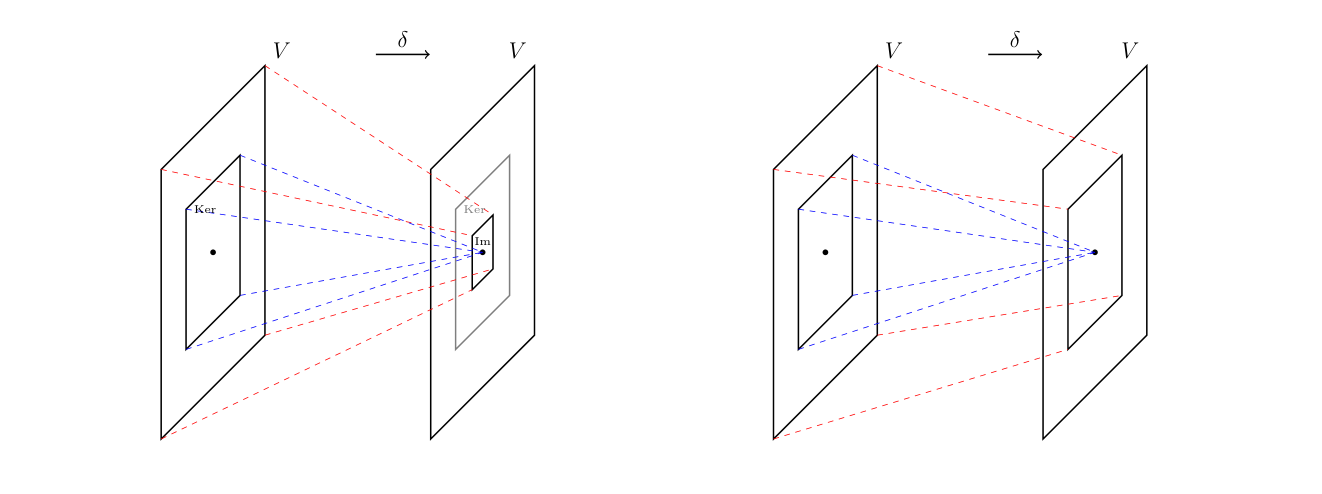
\includegraphics[width=0.8\textwidth]{img/1-cohomology.png}
    \caption{
        The cohomology measures the amount of non-exactness of closed elements. It is mathematically nontrivial when \(\mathrm{Im}(\delta) \subset \mathrm{Ker}(\delta)\). The right-hand side specifically depicts the trivial case of vanishing cohomology, \(\mathrm{Im}(\delta) = \mathrm{Ker}(\delta)\), where all closed elements are exactly exact.
    }
    \label{fig:1-cohomology}
\end{figure}

All the point inside \(\mathrm{Ker}(\delta)\) are mapped to zero by the operator \(\delta\). The image of \(\delta\) is a subspace of \(\mathrm{Ker}(\delta)\), and the cohomology is the quotient space of these two subspaces: it is the ``difference'' of \(\mathrm{Im}(\delta)\) and \(\mathrm{Ker}(\delta)\). When the cohomology is nontrivial, it is mathematically said that there exist closed elements that are not exact. In contrast, when the cohomology is trivial, all closed elements are automatically exact, thus \(\mathrm{Im}(\delta) = \mathrm{Ker}(\delta)\) and the quotient space is empty. In this case, the operator \(\delta\) is said to be \textit{acyclic}.

\subsubsection{Application to the BRST Formalism}

Returning to the BRST construction discussed previously, the \textbf{Slavnov operator} \(s\) serves precisely as a nilpotent operator. It acts dynamically on the functionals of the fields (like the lagrangian and the action), which comprehensively include both ghosts and non-minimal auxiliary fields. \textit{Physical observables} are theoretically defined to be BRST invariant quantities, i.e., they are annihilated by the operator \(s\) that defines the infinitesimal BRST transformations (the BRST symmetry perfectly takes the role of gauge invariance within the gauge-fixed theory). \uline{Physical observables that differ merely by the BRST variation of some other arbitrary quantity must be identified as physically equivalent}: \textit{therefore, physical observables are rigorously defined by the cohomology classes of} \(s\).

For example, the total gauge-fixed action is a nontrivial cohomological element evaluated at vanishing ghost number:
\begin{equation} \label{eq:action_cohomology}
    S \sim S_{tot} = S + s\Psi \, ,
\end{equation}
where \(\Psi\) represents the gauge-fixing fermion.

Similarly, transitioning to canonical quantization, the classical BRST charge \(Q\) becomes a quantum operator \(\hat{Q}\) (on the BRST Hilbert space, since it has a redundant structure including ghosts and auxiliary fields). It is the Noether charge fundamentally associated with the BRST symmetry that becomes an operator upon canonical quantization. It intrinsically possesses the fundamental mathematical properties of being: hermitian (\(\hat{Q}^\dagger = \hat{Q}\)), carrying a ghost number of one, and being strictly nilpotent (\(\hat{Q}^2 = 0\)). Like all conserved charges, such as the Hamiltonian, it plays a profound dual role:
\begin{itemize}
    \item[(i)] it is a rigorously conserved quantity due to an underlying Lie symmetry of the system,
    \item[(ii)] it acts as the algebraic generator of that Lie symmetry on the quantum system under study.
\end{itemize}

Consequently, \textit{physical states are defined by the cohomology of the operator} \(\hat{Q}\) evaluated on the full BRST Hilbert space at vanishing ghost number. That is, \textbf{valid physical states} are given by specific vectors of the Hilbert space at vanishing ghost number that are definitively BRST invariant, and thus satisfy the closed condition
\[
    \hat{Q}\ket{\psi_{ph}} = 0.
\]
In addition to this, physical states are deemed \textbf{equivalent} if they differ solely by the BRST variation of another state: \(\ket{\psi_{ph}}\) and \(\ket{\psi'_{ph}}\) are strictly equivalent if they are related by
\[
    \ket{\psi'_{ph}} = \ket{\psi_{ph}} + \hat{Q}\ket{\chi},
\]
for some arbitrary state \(\ket{\chi}\). Similarly, \textit{physical operators} are defined by cohomology classes: they are BRST invariant operators, meaning that they commute in a graded sense with the BRST charge \(\hat{Q}\), i.e., \([\hat{Q}, \hat{A}_{ph}\} = 0\), and they are subject to an equivalence relation given by
\[
    \hat{A}'_{ph} \sim \hat{A}_{ph} = \hat{A}_{ph} + [\hat{Q}, \hat{B}\},
\]
for some operator \(\hat{B}\).

One may mathematically check that the matrix elements of physical operators evaluated between physical states do not depend on the specific representative chosen in the respective classes of equivalence, namely
\begin{equation} \label{eq:matrix_element_equivalence}
    \langle \psi_{ph} | \hat{A}_{ph} | \phi_{ph} \rangle = \langle \psi'_{ph} | \hat{A}'_{ph} | \phi'_{ph} \rangle \, .
\end{equation}
To explicitly prove this, for example, if we take \(\vert{}\phi'_{ph}\rangle = \vert{}\phi_{ph}\rangle + \hat{Q}\ket{\chi}\), then the modified matrix element expands as
\begin{equation} \label{eq:matrix_expansion}
    \langle \psi_{ph} | \hat{A}_{ph} | \phi'_{ph} \rangle = \langle \psi_{ph} | \hat{A}_{ph} | \phi_{ph} \rangle + \langle \psi_{ph} | \hat{A}_{ph} \hat{Q} | \chi \rangle
\end{equation}
but the last term identically vanishes because both \(\langle \psi_{ph}\vert{}\) and \(\hat{A}_{ph}\) are physical (and thus are annihilated by or commute with \(\hat{Q}\)), so that
\begin{equation} \label{eq:matrix_vanishing_term}
    \langle \psi_{ph} | \hat{A}_{ph} \hat{Q} | \chi \rangle = \langle \psi_{ph} | [\hat{A}_{ph}, \hat{Q}] | \chi \rangle + \langle \psi_{ph} | \hat{Q} \hat{A}_{ph} | \chi \rangle = 0
\end{equation}
where we have deliberately taken \(\hat{A}_{ph}\) to be bosonic for simplicity, meaning the graded commutator reduces to a standard commutator. Thus, we firmly establish that
\begin{equation} \label{eq:matrix_final_equivalence}
    \langle \psi_{ph} | \hat{A}_{ph} | \phi'_{ph} \rangle = \langle \psi_{ph} | \hat{A}_{ph} | \phi_{ph} \rangle \, .
\end{equation}

Finally, it is crucial to note that the full BRST Hilbert space cannot theoretically have a positive-definite norm. For example, exact states constructed like \(\hat{Q}\ket{\chi}\) inherently have a vanishing norm, as demonstrated by
\begin{equation} \label{eq:vanishing_norm}
    |\hat{Q}|\chi\rangle|^2 = \langle \chi | \hat{Q}^\dagger \hat{Q} | \chi \rangle = \langle \chi | \hat{Q}\hat{Q} | \chi \rangle = 0
\end{equation}
where we have explicitly used the hermiticity of \(\hat{Q}\) and its foundational nilpotence. However, this is not a physical problem; it is only theoretically important that the norm restricted to the physical sector of the Hilbert space (the cohomology classes) be positive definite. (\textit{For further details, one may consult chapter 74 of Srednicki.})

\subsection{Application: Gauge-Fixing of Perturbative Quantum Gravity}

A further compelling application of the BRST method lies in the systematic gauge-fixing of the Einstein-Hilbert action for perturbative quantum gravity. In this fundamental theory, the dynamical field is the metric tensor \(g_{\mu\nu}(x)\), which geometrically defines the invariant length element in spacetime:
\begin{equation} \label{eq:line_element}
    ds^2 = g_{\mu\nu}(x)dx^\mu dx^\nu \, .
\end{equation}

The classical dynamics of gravity are governed by the Einstein-Hilbert action:
\begin{equation} \label{eq:einstein_hilbert}
    S_{EH}[g_{\mu\nu}] = \frac{1}{\kappa^2} \int d^4x \sqrt{g} R(g)
\end{equation}
where \(g = |\det g_{\mu\nu}|\) denotes the absolute value of the determinant of the metric, \(R(g)\) is the Ricci scalar uniquely built from \(g_{\mu\nu}\), and the constant \(\kappa^2 = 16\pi G\) incorporates Newton's constant \(G\). The parameter \(\kappa\) is naturally taken as the perturbative coupling constant of the theory. Our mathematical conventions follow directly from the standard definition of the covariant derivative \(\nabla_\mu\), which acts on arbitrary vector fields as:
\[
    \nabla_\mu V^\nu = \partial_\mu V^\nu + \Gamma^\nu_{\mu\rho} V^\rho \, , \qquad \nabla_\mu W_\nu = \partial_\mu W_\nu - \Gamma^\rho_{\mu\nu} W_\rho
\]
where the Christoffel symbols \(\Gamma^\rho_{\mu\nu}\), identifying the components of the unique, torsion-free Levi-Civita connection, are expressed purely in terms of the metric:
\[
    \Gamma^\rho_{\mu\nu} = \frac{1}{2}g^{\rho\sigma}(\partial_\mu g_{\nu\sigma} + \partial_\nu g_{\mu\sigma} - \partial_\sigma g_{\mu\nu}) \, .
\]
Covariant derivatives inherently do not commute when acting on tensors; this non-commutativity is precisely used to define the fundamental curvature tensors:
\begin{equation} \label{eq:curvature_tensors}
    [\nabla_\mu, \nabla_\nu]V^\rho = R_{\mu\nu}{}^\rho{}_\sigma V^\sigma \, , \quad R_{\mu\nu} = R_{\rho\mu}{}^\rho{}_\nu \, , \quad R = g^{\mu\nu}R_{\mu\nu}
\end{equation}
known respectively as the Riemann tensor, the Ricci tensor, and the Ricci scalar. By explicitly calculating the commutator, one finds the explicit formula for the Riemann tensor directly in terms of the connection:
\[
    \begin{aligned}
        R_{\mu\nu}{}^\rho{}_\sigma & = \partial_\mu \Gamma^\rho_{\nu\sigma} - \partial_\nu \Gamma^\rho_{\mu\sigma} + \Gamma^\rho_{\mu\lambda}\Gamma^\lambda_{\nu\sigma} - \Gamma^\rho_{\nu\lambda}\Gamma^\lambda_{\mu\sigma} \\
                                   & = \hat{\nabla}_\mu \Gamma^\rho_{\nu\sigma} - \hat{\nabla}_\nu \Gamma^\rho_{\mu\sigma}
    \end{aligned}
\]
where in the final line, we wrote a highly useful mnemonic notation in which the symbol \(\hat{\nabla}_\mu\) denotes a specialized covariant derivative acting exclusively on the upper index of the associated Christoffel symbols. Using all these geometric relations recursively, one successfully finds the Einstein-Hilbert action as a highly non-trivial functional of the metric, whose stationary variation leads directly to Einstein's field equations in vacuum. Crucially, this action is constructed as a true scalar under any arbitrary change of spacetime coordinates, which thus constitutes the fundamental gauge symmetry of the theory.

\subsubsection{Diffeomorphism Invariance and Perturbative Expansion}

An arbitrary smooth change of coordinates (often referred to formally as a diffeomorphism or reparametrization) mapping old coordinates to new ones:
\[
    x^\mu \rightarrow x'^\mu(x)
\]
dynamically induces a corresponding change in the metric tensor components given by the standard tensorial transformation law:
\begin{equation} \label{eq:metric_transform_finite}
    g_{\mu\nu}(x) \rightarrow g'_{\mu\nu}(x') = g_{\alpha\beta}(x) \frac{\partial x^\alpha}{\partial x'^\mu} \frac{\partial x^\beta}{\partial x'^\nu} \, .
\end{equation}
Under an infinitesimal change of coordinates continuously parametrized by a small vector field \(\xi^\mu(x)\):
\[
    x^\mu \rightarrow x'^\mu = x^\mu - \xi^\mu(x)
\]
the metric transforms at linear order in \(\xi\) as:
\begin{equation} \label{eq:metric_transform_infinitesimal}
    \begin{aligned}
        \delta g_{\mu\nu}(x) & = g'_{\mu\nu}(x) - g_{\mu\nu}(x) = \xi^\rho(x)\partial_\rho g_{\mu\nu}(x) + \partial_\mu \xi^\rho(x) g_{\rho\nu}(x) + \partial_\nu \xi^\rho(x) g_{\mu\rho}(x) \\
                             & = \nabla_\mu \xi_\nu(x) + \nabla_\nu \xi_\mu(x)
    \end{aligned}
\end{equation}
as can be directly deduced from expanding the finite transformation rule given above. Consequently, there are exactly four independent gauge functions contained within the infinitesimal vector field \(\xi^\mu\).

Perturbatively, to study small fluctuations of gravity around a flat Minkowski background spacetime, one systematically splits the full metric as:
\begin{equation} \label{eq:metric_perturbation}
    g_{\mu\nu}(x) = \eta_{\mu\nu} + \kappa h_{\mu\nu}(x)
\end{equation}
where \(h_{\mu\nu}(x)\) is the dynamical field whose quantized quanta are physically identified as ``gravitons''. The complete action, when expanded as a power series in terms of the fluctuation field \(h_{\mu\nu}(x)\), contains a leading quadratic part which formally identifies the free graviton propagator (only after an appropriate gauge-fixing procedure), plus an infinite number of interaction vertices:
\[
    S_{EH}[g_{\mu\nu}] = S_2[h_{\mu\nu}] + \sum_{n=3}^\infty S_n[h_{\mu\nu}] \, .
\]
The full Einstein-Hilbert action is highly nonlinear in \(h_{\mu\nu}(x)\), meaning that interaction vertices of any arbitrary order \(n\) are fundamentally present in the theory. These vertices possess a quite complicated algebraic structure, but the free quadratic part is relatively easy to derive (see appendix). However, this quadratic part inherently contains a kinetic differential operator that is strictly non-invertible precisely because of the underlying gauge symmetry shown in Eq. (\ref{eq:metric_transform_infinitesimal}). Thus, one absolutely cannot obtain the propagator for \(h_{\mu\nu}\) directly, and a rigorous gauge-fixing procedure is unavoidably required.

\subsubsection{BRST Transformations for Gravity}

Let us now meticulously apply the BRST method to this system. To start with the BRST quantization of the action in Eq. (\ref{eq:einstein_hilbert}), we first introduce the fermionic ghost field \(c^\mu\) by effectively replacing the local gauge parameters \(\xi^\mu(x) \rightarrow \Lambda c^\mu(x)\), and we logically define the fundamental BRST rule on the full metric \(g_{\mu\nu}\) by extending the infinitesimal transformation:
\begin{equation} \label{eq:brst_metric}
    \delta_B g_{\mu\nu} = \Lambda(\nabla_\mu c_\nu + \nabla_\nu c_\mu) \, .
\end{equation}
The strict mathematical requirement of nilpotency (\(s^2 = 0\)) uniquely fixes the corresponding BRST transformation rule for the ghost fields themselves:
\begin{equation} \label{eq:brst_ghost}
    \delta_B c^\mu = \Lambda c^\nu \partial_\nu c^\mu \, .
\end{equation}
The direct calculation to prove this is algebraically quite lengthy, but recognizing the underlying geometrical considerations vastly simplifies the task. To that distinct purpose, let us notice that the classical gauge symmetry is mathematically generated by Lie derivatives taken along the vector field \(\xi^\mu\) (conventionally denoted by \(\mathcal{L}_\xi\)). This insight gracefully translates into the fact that the transformation in Eq. (\ref{eq:metric_transform_infinitesimal}) may be compactly rewritten as:
\[
    \delta g_{\mu\nu} = \mathcal{L}_\xi g_{\mu\nu}
\]
(this mathematical formulation actually defines the Lie derivative on the metric tensor). More generally, any arbitrary tensor geometrically transforms under the infinitesimal change of coordinates given in Eq. (\ref{eq:metric_transform_infinitesimal}) by its Lie derivative evaluated along \(\xi^\mu\). In particular, a simple scalar field \(\phi\) transforms smoothly as:
\[
    \delta\phi = \mathcal{L}_\xi \phi = \xi^\mu \partial_\mu \phi
\]
which would naturally dictate a BRST transformation of the form:
\[
    \delta_B \phi = \Lambda c^\mu \partial_\mu \phi \, .
\]
It is significantly simpler to study the nilpotency condition explicitly on the scalar \(\phi\) in order to uniquely fix the BRST rule of the ghosts. This procedure amounts conceptually to extracting the fundamental structure constants of the infinite-dimensional algebra of diffeomorphisms. Writing \(\delta_B c^\mu = \Lambda s c^\mu\) in terms of the abstract Slavnov variation \(s\), we strictly impose nilpotency:
\[
    s^2\phi = s(c^\mu \partial_\mu \phi) = s c^\mu \partial_\mu \phi - c^\mu \partial_\mu (c^\nu \partial_\nu \phi) = s c^\mu \partial_\mu \phi - c^\mu (\partial_\mu c^\nu)\partial_\nu \phi
\]
that unambiguously fixes the variation of the ghost field to be:
\begin{equation} \label{eq:slavnov_ghost}
    s c^\mu = c^\nu \partial_\nu c^\mu \quad \longrightarrow \quad \delta_B c^\mu = \Lambda c^\nu \partial_\nu c^\mu \, .
\end{equation}
This specific rule elegantly captures the structure constants carried intrinsically by the commutator of the Lie derivatives:
\begin{equation} \label{eq:lie_algebra_diffeo}
    [\mathcal{L}_\xi, \mathcal{L}_\eta] = \mathcal{L}_{[\xi,\eta]}
\end{equation}
which precisely forms the underlying gauge algebra of the group of diffeomorphisms. Thus, we have successfully found the complete set of BRST transformations that inherently contain the deep geometrical information on the structure constants of the gauge group:
\begin{equation} \label{eq:brst_complete_gravity}
    \begin{aligned}
        \delta_B g_{\mu\nu} & = \Lambda(\nabla_\mu c_\nu + \nabla_\nu c_\mu) \\
        \delta_B c^\mu      & = \Lambda c^\nu \partial_\nu c^\mu \, .
    \end{aligned}
\end{equation}

\subsubsection{Gauge-Fixing and the Total Action}

Now, to properly implement a robust gauge-fixing procedure, we add the standard non-minimal fields \(\bar{c}_\mu\) (antighost) and \(B_\mu\) (Nakanishi-Lautrup auxiliary field) which strictly possess trivial BRST transformations:
\[
    \begin{aligned}
        \delta_B \bar{c}_\mu & = \Lambda B_\mu \\
        \delta_B B_\mu       & = 0 \, .
    \end{aligned}
\]
A particularly convenient gauge choice utilizes the specific functions:
\begin{equation} \label{eq:de_donder_gauge}
    f^\mu = \partial_\nu(\sqrt{g} g^{\nu\mu})
\end{equation}
which, when set to zero, efficiently fix the harmonic gauge (widely known in gravity literature as the de Donder gauge). We thoughtfully use this condition to construct the gauge fermion density:
\begin{equation} \label{eq:gauge_fermion_gravity}
    \psi = \frac{1}{\kappa^2} \bar{c}_\mu \left( \partial_\nu(\sqrt{g} g^{\nu\mu}) + \alpha g^{\mu\nu} B_\nu \right)
\end{equation}
which mathematically possesses the desirable property of identifying a particularly simple and invertible graviton propagator for a specific tuning of the arbitrary gauge parameter \(\alpha\).

At this final stage, we have successfully constructed the full gauge-fixed action for pure quantum gravity, which is elegantly given by:
\begin{equation} \label{eq:total_action_gravity}
    S_{tot} = S_{EH} + s\Psi
\end{equation}
with the integrated gauge-fixing fermion \(\Psi = \int d^4x \, \psi\). This total effective action is manifestly BRST invariant by construction. It rigorously serves as the essential starting point for any consistent perturbative treatment of quantum gravity.

\subsection{Graviton Propagator in Flat Spacetime}

The total gauge-fixed gravitational action derived previously is algebraically quite complex, and standard perturbative calculations in quantum gravity are notoriously difficult.

Let us systematically work out some details by carefully keeping only the quadratic approximation in the metric fluctuation \(h_{\mu\nu}\). This approximation directly leads to the perturbative propagator of the graviton (and its corresponding ghosts). Expanding the Einstein-Hilbert action strictly to quadratic order in the fluctuation field \(h_{\mu\nu}\), one explicitly finds\footnote{Detailed mathematical steps for this calculation may be found in Appendix A.}:
\begin{equation} \label{eq:action_quadratic}
    S_2[h] = \int d^4x \left[ \frac{1}{4} h^{\mu\nu}\partial^2 h_{\mu\nu} - \frac{1}{8} h\partial^2 h + \frac{1}{2} \Big( \partial^\nu h_{\nu\mu} - \frac{1}{2} \partial_\mu h \Big)^2 \right]
\end{equation}
with the trace defined as \(h \equiv \eta^{\mu\nu}h_{\mu\nu}\). Here, the raising and lowering of indices is consistently done using only the flat Minkowski background metric \(\eta_{\mu\nu}\). As detailed in the appendix, we have redefined the fluctuation field via \(h_{\mu\nu} \rightarrow \kappa h_{\mu\nu}\) to absorb the coupling constant, and we use a completely similar redefinition for the corresponding ghosts, auxiliary field, and local gauge parameters to ensure canonical kinetic terms.

This quadratic free action dynamically possesses a gauge symmetry under the specifically linearized version of the full diffeomorphism transformation, which at lowest order cleanly reads:
\begin{equation} \label{eq:linearized_gauge_sym}
    \delta h_{\mu\nu}(x) = \partial_\mu \xi_\nu + \partial_\nu \xi_\mu
\end{equation}
with the lowered parameter defined as \(\xi_\mu = \eta_{\mu\nu}\xi^\nu\). The de Donder gauge-fixing function utilized previously smoothly linearizes to the precise condition:
\begin{equation} \label{eq:linearized_gauge_fix}
    f^\mu = -\Big( \partial_\nu h^{\nu\mu} - \frac{1}{2} \partial^\mu h \Big)
\end{equation}
which, once successfully inserted into the definition of the gauge fermion
\begin{equation} \label{eq:gauge_fermion_linear}
    \psi = \bar{c}_\mu(f^\mu + \alpha B^\mu) \, ,
\end{equation}
systematically gives rise to a BRST variation of the form:
\begin{equation} \label{eq:brst_variation_linear}
    s\psi = B_\mu(f^\mu + \alpha B^\mu) + \bar{c}_\mu \partial^2 c^\mu \sim -\frac{1}{4\alpha} f^2 + \bar{c}_\mu \partial^2 c^\mu
\end{equation}
where in the very last expression, the algebraic \(B_\mu\) equations of motion have been explicitly used to eliminate the auxiliary field. By smartly setting the gauge parameter to \(\alpha = \frac{1}{2}\), one elegantly obtains the absolute simplest form of the total gauge-fixed action (this specific choice ensures the term containing \(f^2\) will exactly cancel the problematic last term in Eq. (\ref{eq:action_quadratic})), and we cleanly find:
\begin{equation} \label{eq:total_quadratic_action}
    S_{2,tot} = S_2[h] + s\Psi = \int d^4x \left( \frac{1}{4} h^{\mu\nu}\partial^2 h_{\mu\nu} - \frac{1}{8} h\partial^2 h + \bar{c}_\mu \partial^2 c^\mu \right) \, .
\end{equation}

With this vastly simplified action, it is now a simple, straightforward algebraic matter to derive the momentum-space propagators. The quadratic lagrangian specifically for the graviton field \(h_{\mu\nu}\) is elegantly cast as:
\begin{equation} \label{eq:lagrangian_quadratic_cast}
    \mathcal{L}_h = \frac{1}{2} h_{\mu\nu} \tilde{P}^{\mu\nu, \alpha\beta} \partial^2 h_{\alpha\beta}
\end{equation}
in terms of the highly symmetric kinetic tensor:
\begin{equation} \label{eq:kinetic_tensor}
    \tilde{P}^{\mu\nu, \alpha\beta} = \frac{1}{4} ( \eta^{\mu\alpha}\eta^{\nu\beta} + \eta^{\mu\beta}\eta^{\nu\alpha} ) - \frac{1}{4} \eta^{\mu\nu}\eta^{\alpha\beta}
\end{equation}
which, when evaluated in an arbitrary spacetime dimension \(D\), mathematically possesses a well-defined inverse given by:
\begin{equation} \label{eq:kinetic_inverse}
    P_{\mu\nu, \alpha\beta} = ( \eta_{\mu\alpha}\eta_{\nu\beta} + \eta_{\mu\beta}\eta_{\nu\alpha} ) - \frac{2}{D-2} \eta_{\mu\nu}\eta_{\alpha\beta}
\end{equation}
that strictly satisfies the defining inversion relation:
\begin{equation} \label{eq:inverse_identity}
    \tilde{P}^{\mu\nu, \alpha\beta} P_{\alpha\beta, \rho\sigma} = \frac{1}{2}( \delta^\mu_\rho \delta^\nu_\sigma + \delta^\nu_\rho \delta^\mu_\sigma ) \, .
\end{equation}

The fundamental physical propagators are then given directly by:
\begin{equation} \label{eq:propagators_gravity}
    \begin{aligned}
        \langle h_{\mu\nu}(x) h_{\alpha\beta}(y) \rangle & = \int \frac{d^D p}{i(2\pi)^D} \, e^{ip(x-y)} \frac{P_{\mu\nu, \alpha\beta}}{p^2 - i\epsilon} \\
        \langle c_\mu(x) \bar{c}_\nu(y) \rangle          & = \int \frac{d^D p}{i(2\pi)^D} \, e^{ip(x-y)} \frac{\eta_{\mu\nu}}{p^2 - i\epsilon} \, .
    \end{aligned}
\end{equation}
These derived formulas are perfectly valid in arbitrary spacetime dimensions \(D\), but of course, for standard physical applications, one can smoothly set directly \(D = 4\).